\documentclass[10pt,lettersize,journal]{IEEEtran}
\usepackage{fontspec}
\setmainfont[BoldFont=texgyretermes-bold.otf,ItalicFont=texgyretermes-italic.otf,BoldItalicFont=texgyretermes-bolditalic.otf]{texgyretermes-regular.otf}
\usepackage{amsmath,amssymb,graphicx,booktabs,url}
\usepackage{cite}
\usepackage[hidelinks]{hyperref}
\newsavebox{\uploadedtablebox}
\title{Regional Complementarity and Learned Weighting for Occluded Face Verification}
\author{Sangiya Pararajasingham\thanks{Independent Researcher. ORCID: 0009-0005-3407-2154.}}
\begin{document}
\maketitle
\begin{abstract}
We explore the complementary nature of different facial regions in occluded face verification. Multiple DINOv2 fusion approaches, including no fusion, fixed fusion, and learned fusion, were employed. Five model configurations were trained; frozen encoders with trained projection layers, full face LoRA, periocular LoRA, and dual branch models with equal fusion weights/learned fusion. All models were trained with three seeds on the identity-disjoint ROF training split (4405 of 6171 manifest images) and evaluated using frozen ROF, MFR2, and RMFRD verification protocols. The best performance for masked data was found in the periocular LoRA model (0.9221 \ensuremath{\pm} 0.0046). For sunglasses, the best performance was with the fixed fusion approach (0.8950 \ensuremath{\pm} 0.0021). Neutral data had the best performance in the learned fusion model (0.9458 \ensuremath{\pm} 0.0026). With learned fusion, 0.9548 \ensuremath{\pm} 0.0022 performance was achieved in 802 MFR2 pair comparisons after a known training-name overlap was excluded. Fixed fusion achieved best performance (0.7240 \ensuremath{\pm} 0.0099) from 21798 RMFRD pair comparisons with exact content duplicates removed. When ensuring that the branches in the model were consistently trained, a varying weighted fusion does not guarantee performance gains over a constant weighted fusion. Validation-calibrated thresholds reveal shifts in test false acceptance rates that retrospective AUC summaries do not establish. Separate aligned-SFace and shared-crop SFace evaluations show sensitivity to preprocessing; their AUCs do not establish architectural superiority. Evidence of complementary data in different conditions is provided. We show that using learned fusion gates with high AUCs alone does not guarantee~reliable performance in \mbox{occluded verification}.\par
\end{abstract}
\begin{IEEEkeywords}
Face verification, occlusion robustness, masked face verification, periocular, DINOv2, LoRA, learned fusion, cross dataset.\par
\end{IEEEkeywords}
\section{Introduction}
Face verification determines if two images represent the same individual. In cases where there are occlusions, in either probe or enrolment, the appearance of the face will change. Masked faces result in reduced information from the bottom half of the face. Sunglasses result in reduced information from the eyes and surrounding skin. Therefore, information can be lost between different types of occlusion. Controlling false acceptance rates is crucial in such scenarios.\par
While periocular regions allow for some top of face information in the masked scenarios, there may be useful features within the neutral images. The periocular regions lose information when sunglasses obscure the eyes. Therefore, using both full face and periocular representations seems reasonable. However, having multiple branches in a network does not mean that learning how to best fuse them will lead to improved verification performance.\par
Multiple different representations were tested. Different models include (1) Frozen full face representation, with learned projection; (2) Full face with LoRA; (3) Periocular with LoRA; (4) Two branch model with equal weighting; and (5) Learned fusion. All 5 configurations were independently trained and used the same frozen verification pairs for evaluation. Three seeds were used in training these models. The raw scores and signatures can be followed to see the results. This was done to understand what factors (adaptation, region choice, and fusion) improve performance.\par
As different weights are applied in the fixed and gated fusion models, different features are being learnt in each branch. By applying different weights to the gated models, but keeping the same branches, it was found that equal weighting in the gated branches performs better than learned weighting in masked ROF pairs.\par
To address issues in historical data, one image with an exact content duplication within training and validation sets was removed. One near duplicate image with different labels in training and testing was also removed. After retraining on the cleaned ROF manifest, external evaluation excluded the known exact-name overlap between MFR2 and ROF training and the recorded cross-label exact-content conflicts in RMFRD. This means that certain issues have been addressed in the data. However, we cannot be confident that all semantically meaningful labels are valid, nor that data is independent from backbone pre-training.\par
Three key findings were observed. First, comparisons between configurations across different seeds help distinguish effects of adaptation, region selection, and fusion in fixed pairs. Second, changing the weights within the same branches allows us to understand if improved performance in learned representations is due to the inference weighting rule. Third, thresholding based on validation data, sensitivity to identity removal and using shared-crop face-recognition models as controls indicate that limitations in performance exist beyond what would be obvious from comparing AUCs. Overall, improvements in replicability have been made. However, it is not novel to perform adaptation in DINOv2 models \cite{dinov2} using LoRA \cite{lora}, nor to exploit complementary information between full face and periocular representations.\par
\section{Related Work}
\subsection{Face verification}
Embeddings are learnt such that images of the same individual cluster together. Distinct individuals should be separated. Cosine similarity between embeddings is commonly used as it is easy to implement, invariant to scaling (once normalised) and is compatible with ROC analysis. Improvements in clean face verification benchmarks have been made by employing margin based losses. SphereFace uses a multiplicative angular margin \cite{sphereface}, CosFace uses an additive margin in cosine similarity \cite{cosface} and ArcFace uses additive margin in the hypersphere \cite{arcface}. AdaFace allows for adaptive margins dependent on image quality \cite{adaface}. MagFace also incorporates adaptive margins, depending on embedding magnitude to reflect quality \cite{magface}. During training, only known identities are optimised. In ROF verification, unknown identities are verified. In external protocols, limits on identity overlap are imposed.\par
\subsection{Masked and occluded face recognition}
Since the beginning of the pandemic, masked face recognition has become an area of specific interest. Masked face simulation (MaskTheFace) and masked face datasets (MFR2) were introduced \cite{mfr2}. MAFA/LLE-CNNs were proposed by Ge et al. to detect masked faces \cite{llecnn}. Wang et al. created a series of masked face datasets (MFDD, RMFRD, SMFRD) \cite{rmfrd}. A review of occlusion robust face recognition approaches was conducted in 2021 \cite{surveyocc}. Recently, dynamic masking of corrupted features \cite{from2022}, pairwise differential Siamese mask learning \cite{masklearn} and self restrained triplet loss to unmask face embeddings \cite{umr} have been proposed. A multi task contrastive learning approach was proposed by Neto et al. called FocusFace \cite{focusface}. Neto et al. also analyse generalisability of masked face models to broader occlusions \cite{beyondmasks}. Strong results have been found using real masked face datasets. Strong results were achieved in IJCB competition in MFR 2021 \cite{mfr2021}, and in the InsightFace track \cite{insightfacemfr}. Training models on synthetic masked faces and testing on real masks has been investigated by Hsu et al. \cite{hsu2022}. Real upper (sunglasses) and lower (mask) occlusions, with specific evaluation protocols, exist in the ROF dataset \cite{rof}. Recently, direct complementary information between face and periocular representations has also been considered. Attention and prompting are used to learn aligned face and periocular representations in Flexible Biometrics Recognition \cite{fbr2024}. This is especially applicable to this work as complementary information between these two regions was considered.\par
\subsection{Periocular recognition}
Periocular biometric information can be extracted. Both visible spectrum periocular comparison (including eyebrow information) and merging face and periocular information were considered by Park, Jillela, Ross, and Jain \cite{periocular}. Recently, consistent knowledge distillation has been applied to allow periocular embeddings to be trained from full face data. This means useful information can be passed to periocular embeddings even if only periocular data is available at inference time \cite{ckd2024}. Periocular recognition is therefore a suitable option to handle lower occlusions. However, sunglass occlusions impact the periocular region.\par
Recently, Alonso-Fernandez et al. trained periocular networks using ocular cropped regions from large face datasets \cite{ocularcrop2025}. This highlights the importance of considering the size of training data, how cropping is performed, and acquisition protocol between full face and periocular models. However, results cannot be directly compared between this method of verification and fixed pair verification in ROF. Prasad et al. used LoRA adapted DINOv2 models with quality aware fusion of enrolment templates to enable cross spectral periocular recognition \cite{perilora2026}. In contrast, in this work, the weighting between full face and periocular branches in visible spectrum occlusions is explored. Constant auxiliary inputs and negative gate controls are employed. While it is not novel to apply DINOv2 with LoRA in periocular recognition, nor the quality aware fusion approach, this work is not the first to consider periocular recognition with DINOv2 and LoRA.\par
\subsection{Pretrained visual representations}
DINOv2 creates transferable features from 142M self-supervised images \cite{dinov2}. DINO is a vision transformer model \cite{dino}. MAE reconstructs masked patches \cite{mae}, SimCLR maximises agreement between positive augmented views of the same image \cite{simclr} and CLIP is trained with image text supervision \cite{clip}. These approaches are not compared to in this work. DINOv2 and CLIP have already been adapted to face identification using LoRA \cite{froundation2025}. Therefore applying LoRA to visual face encoders is not novel. General and face specific models were compared by Sony et al. and it was found that fusion and contextual cropping is important \cite{foundationcomparison2025}. This motivates separation of preprocessing, adaptation and fusion in this diagnostic baseline model.\par
\subsection{Parameter-efficient adaptation}
LoRA allows efficient adaptation in language models by learning low rank updates without modifying the original parameters \cite{lora}. In this work, LoRA is applied to a visual encoder. Prompt tuning in vision (VPT) allows prompt tokens to be learnt for frozen vision transformers \cite{vpt}. In frozen language models, soft prompts have been researched \cite{prompt}. However, this is not tested in this work. Light adapters can be applied to frozen pre-trained backbones in vision to adapt them \cite{adaptformer}. However, in this work, LoRA is preferred as attention projections can be directly adapted, and fits well with the DINOv2 backbone.\par
\subsection{Score fusion and quality-aware gating}
Score fusion in biometrics has been heavily studied. Ross and Jain studied score fusion in matching \cite{fusionRossJain}. Scores can be processed and fused depending on their quality to utilise useful information within samples \cite{quality}. Weights in fusion can be learnt in order to depend on cues specific to each sample. In this work, a gate is learnt such that branch outputs are weighted according to branch embeddings and auxiliary slot inputs. As constant inputs were applied in this experiment, the gate is not demonstrably quality aware. However, unlike margin adaptive losses \cite{magface,adaface}, this gate is applied to the fusion of embeddings, and not the training of the classifier.\par
\section{Research Questions and Hypotheses}
RQ1: How much improvement is achieved by identity supervised LoRA adaptation compared to the frozen full face with trained projection baseline? RQ2: When is the periocular representation useful? What is lost in periocular representations alone? RQ3: Is performance improved by learned weighting compared to equal weighting? Does this improvement occur in ROF, MFR2, and RMFRD?\par
H1: Full face LoRA model will achieve better performance than frozen projection baseline. H2: Periocular adaptation will be beneficial in masks. However, information may be lost in sunglasses/neutral conditions. H3: Learned fusion will achieve better performance in certain low FAR points. These hypotheses were tested in ablation studies. Even if the expected improvements were not observed, results were still reported. Comparing AUC values and conducting calibration analysis investigates slightly different questions to hypothesis 3, therefore increased AUC values are not considered sufficient evidence of hypothesis 3.\par
\section{Methods}
\subsection{Branch representations}
Let \ensuremath{x_f} and \ensuremath{x_p} be full face and periocular data. \ensuremath{x_p} contains both eyes, eyebrows, top of nose and local context. \ensuremath{E_f} and \ensuremath{E_p} are DINOv2 encoders, and \ensuremath{P_f} and \ensuremath{P_p} are learnable projection heads. Normalised branch outputs are:\par
\begin{equation}
z_f=\operatorname{norm}(P_f(E_f(x_f))),\quad z_p=\operatorname{norm}(P_p(E_p(x_p))).
\end{equation}
Branches are the same resolution and normalised. If landmarks cannot be detected in a cropped image, this is recorded in the manifest. However, images are not replaced with full face images.\par
The gated-fusion inference architecture is shown only in Supplemental Fig. S1; the identity classifier is used only during training.\par
\subsection{Fixed and learned fusion}
The fixed fusion operation performs equal weighting.\par
\begin{equation}
z_{\mathrm{fixed}}=\operatorname{norm}(0.5z_f+0.5z_p).
\end{equation}
Within the learned fusion model, a weighting factor is learned.\par
\begin{equation}
g=\sigma\!\left(\operatorname{MLP}([z_f;z_p;q_f;q_p])\right),
\end{equation}
\ensuremath{q_f} and \ensuremath{q_p} are auxiliary descriptor slots. Within this experiment, these are kept constant. The final embedding is:
\begin{equation}
z_{\mathrm{gate}}=\operatorname{norm}(gz_f+(1-g)z_p).
\end{equation}
Although a gate is used in this model, it is considered a learned fusion approach. Four auxiliary descriptors and branch embeddings are input to the gate. However, during all new training and evaluation, the vector was kept constant [1,0,0,1]. In previous experiments, issues were found with the auxiliary inputs and key caching. However, this does not affect the key results of this experiment. Therefore, we do not claim the scalar value of the gate is calibrated with quality. Since the auxiliary input is constant, a constant bias is added in the first layer of the gate. Therefore, if the gate varies, this must be related to variations in the branch embeddings. Distribution of weights and replacement of learned weights explores this relationship.\par
\subsection{Training objective}
The LoRA parameters are added to certain attention projection layers. The encoder parameters are kept fixed during training. The LoRA parameters and projection/ fusion heads are optimised. For embedding \ensuremath{h_i} and training identity \ensuremath{y_i}, the per-image cross-entropy is:\par
\begin{equation}
\ell_i=-\log p(y_i\mid h_i).
\end{equation}
Only training identities define the classifier classes. EER’s and control TAR’s are calculated using the ROC curves retrospectively. Thresholds are chosen based on identities from the validation set. Once thresholds have been chosen they remain fixed. The true TAR and FAR values are given. The score for verifying two normalised embeddings (i,j) is:\par
\begin{equation}
s(i,j)=z_i^{\top}z_j.
\end{equation}
\subsection{Model configurations}
Ablations are performed to analyse adaptation, region selection and fusion in the models. In M0, the projection has been trained but encoder is fixed.\par
\begin{table}[t]\centering
\caption{Model Comparison}
\label{tab:checked1}
\footnotesize\setlength{\tabcolsep}{2pt}
\sbox{\uploadedtablebox}{\begin{tabular}{ll}\toprule
Model & Comparison\\\midrule
M0 & Frozen encoder, trained projection Baseline heads\\
M1 & Full face DINOv2 + LoRA Adaptation\\
M2 & Periocular DINOv2 + LoRA Periocular only\\
M3 & Two LoRA, fixed fusion No gate\\
M4 & Two LoRA, learned gate Fusion\\
\bottomrule\end{tabular}}
\ifdim\wd\uploadedtablebox>\columnwidth\resizebox{\columnwidth}{!}{\usebox{\uploadedtablebox}}\else\usebox{\uploadedtablebox}\fi
\end{table}
\section{Datasets and Protocol}
\subsection{ROF content and identity audit}
There were 7751 indexed files, 399 condition-specific labels, 182 normalised identity names and 6491 unique hashes. A resource illustration previously indexed as an identity was removed. The number of images in this dataset does not match with published data. All 437 annotated pickles match the blob hashes in the git repository. However, no log of image download history could be found. As such it cannot be confirmed that all images downloaded are valid or that all identities have semantically meaningful labels.\par
Suffixes attached to conditions were normalised before grouping by identity. From the original complete manifest, there were 7295 rows. There were 4 duplicated rows between training and validation data, with differing identity names. On further perceptual analysis, a near duplicate image with differing names was found between training and testing data. Despite having differing file hashes, this image differed slightly in content. In the new manifest, exact duplicates, unreadable content, conflicting labels, and both copies of the confirmed near duplicate image between splits have been removed. The new manifest contains 6171 rows (4405 training, 844 validation, 922 test). Within training, validation and testing, there are 128, 26, and 28 normalised identity labels respectively. File hashes were confirmed to be unique and identity labels disjoint before training. The manifest hash was recorded in all new checkpoints. Historical checkpoints were not continued within this experiment.\par
Each eligible identity and condition had one neutral enrolment image. Self-image comparisons were excluded. 423 comparisons were made in the masked testing protocol, with 47 genuine comparisons, and 376 impostor comparisons. 9 eligible identities were present. Within the sunglasses testing protocol, 6648 comparisons were made with 277 genuine comparisons, and 6371 impostor comparisons. 24 eligible identities in the sunglasses protocol. Within the neutral testing protocol, 15960 comparisons were made, with 570 genuine comparisons, and 15390 impostor comparisons. 28 eligible identities in the neutral protocol. The same comparisons were made in all models. In validation, comparisons were made only with images belonging to validation identities. 300 masked comparisons, 5148 sunglasses comparisons, and 14404 neutral comparisons. Within masked validation, 30 genuine comparisons and 270 impostor comparisons were made with 10 eligible identities. Due to few identities within validation data, generalisations of results are difficult to make.\par
\subsection{External protocols after recorded exclusions}
Within the full MFR2 protocol, 820 comparisons were made. One MFR2 name (Joe Biden) exactly matched one name in ROF’s training data (18 comparisons). Removing these comparisons leaves 802 comparisons (406 genuine, 396 impostors) in this evaluation. Therefore, no known exact-name overlap remains. However, it is unknown whether aliasing, unknown identities, or overlap with pre-training has occurred. No images from MFR2 were used in new gradient updates or thresholding.\par
In the source index of RMFRD, 91849 entries exist. 22554 comparisons were made in exploratory verification. 756 comparisons were affected by exact-content conflicts across nominal identities (36 groupings). Removing these means that there are 21798 comparisons left in this protocol (1038 genuine, 20760 impostors). Therefore, this is an exact content excluded exploratory verification protocol. It is not a benchmark of independently verified semantically meaningful identities. Perceptual duplicates and mislabelled images may still exist. Since a constant auxiliary vector was used for all protocols, it cannot be claimed that a lack of quality metadata in external datasets indicates poor image quality.\par
\subsection{Metrics, calibration, and uncertainty}
Performance metrics have been given as AUC, EER, and TAR (FAR \ensuremath{\leq} \ensuremath{10^{-2}} and \ensuremath{10^{-3}} ). These metrics have been calculated on test data and do not reflect deployment thresholds. All values have been recalculated from raw scores with 10 decimal places of precision. Minimum FAR (non-zero) on masked data: \ensuremath{1/376\approx0.00266}. Therefore, the \ensuremath{10^{-3}} summary only covers a portion of the finite ROC curve with no false accepts. It does not imply a population FAR below \ensuremath{10^{-3}}.\par
Thresholds were chosen to have at most \ensuremath{\lfloor\alpha N_{\mathrm{val}}^{-}\rfloor} false accepts in validation data. In the case of ties, the next highest representable threshold was used. The threshold is then fixed in the corresponding testing conditions for ROF. MFR2 and RMFRD data were tested with the masked validation threshold derived from ROF data (external calibration not performed). The true number of false/true acceptance, FAR and TAR are given. A validation target does not establish the FAR achieved on the test set. With a desired FAR of \ensuremath{10^{-3}} in masked validation, 0 false accepts in validation are allowed (\ensuremath{N_{\mathrm{val}}^{-}=270}).\par
The variance in results from random seeds can be seen by calculating the mean and sample standard deviation in results from 3 independent seeds (7, 42, 123). Sensitivity was analysed using 1000 bootstrap samples. Multinomial sampling was carried out on identity nodes (seed 42). In a bootstrap sample, if identity i is sampled ci times, edges between identities of the same identity will be weighted by ci. Edges between impostor identities i and j will be weighted by cicj. This accounts for identities being sampled multiple times on either side of an edge. In pairwise comparisons, edge weights were applied identically to both systems. Weighting was applied to all 3 fixed seed trainings. Differences in AUC were taken as averages for each bootstrap sample. This gives a percentile range depending on trained checkpoints and selected identities. This range does not indicate uncertainty in all possible training combinations or guarantees to population security. 10 comparisons are given. No claims of significant differences due to multiple comparisons have been made.\par
\section{Experimental Settings}
\subsection{Model settings}
Cropped face and periocular modalities were scaled to 224x224. Normalisation was applied using ImageNet channel statistics. LoRA was applied to the ViT-B/14 DINOv2 backbone (projection dimension = 768). LoRA parameters: r=8, s=16, dropout = 0.1. LoRA updates were applied to QKV projections. Base model parameters were fixed.\par
\subsection{Training settings}
All 15 models were trained on the CPU. 8 threads of PyTorch. 5 full epochs. Batch size = 16, AdamW optimiser, learning rate = 1e-4, weight decay = 1e-4. Cross Entropy loss. 128 labels from training were used within loss calculation. During each epoch, 4405 samples were sampled with replacement (276 batches). 1380 optimisation steps were performed. With research runs, no maximum batch counts were imposed. Classifier heads trained during training were not considered during verification. Final checkpoints from epoch 5 were used. Best epochs were not selected based on test performance.\par
\subsection{Execution environment}
Execution environment: PyTorch (version 2.14.0+cpu), deterministic. DINOv2 was cached.\par
\section{Results}
All results given below are from 15 newly trained models under the deduplication manifest. Historical numerical files are kept for auditing, and were not combined with new runs. Differences in new results from previous full case results and post-hoc filtered results are highlighted.\par
\subsection{Masked ROF verification}
The best results for masked ROF are achieved with periocular LoRA (mean AUC 0.9221). Fixed fusion models give (mean AUC 0.9134) and gated models (mean AUC 0.8989). Full face LoRA performs better than frozen projection baseline models (mean AUC 0.8852 vs 0.8303). This suggests that adaptation improves performance, and that focussing on upper facial features may be beneficial when lower regions are occluded. However, gated models do not perform best in the case of periocular only. The mean difference in performance between gated models and fixed fusion models is -0.0145. The 95\% sensitivity interval from identity resampling is -0.0560 to 0.0144. Only 9 identities exist in the masked testing, meaning a large sensitivity interval. Conditional comparisons can be made.\par
Values in low FAR columns should be treated carefully. For example, even if 0 false acceptances are observed at a test ROC point, TAR may not be 0. It may not be possible to achieve operating points below the first non-zero FAR. In seed=42, operating points with 0 FAR have been omitted. However, these have been included in metric calculation.\par
\begin{table}[t]\centering
\caption{New results from masked ROF. 47 genuine comparisons, 376 impostor comparisons. Mean values given with standard deviation in subscript. 3 seeds. TAR values represent a summary from ROC curves. They do not represent calibrated test rates from validation.}
\label{tab:checked3}
\footnotesize\setlength{\tabcolsep}{2pt}
\sbox{\uploadedtablebox}{\begin{tabular}{lllll}\toprule
Configuration & AUC & EER & TAR 0.01 & TAR 0.001\\\midrule
Frozen + Projection & \shortstack{0.8303\\\ensuremath{\pm}0.024} & \shortstack{0.2580\\\ensuremath{\pm}0.035} & \shortstack{0.1348\\\ensuremath{\pm}0.033} & \shortstack{0.0000\\\ensuremath{\pm}0.000}\\
Whole LoRA & \shortstack{0.8852\\\ensuremath{\pm}0.005} & \shortstack{0.1711\\\ensuremath{\pm}0.004} & \shortstack{0.2553\\\ensuremath{\pm}0.043} & \shortstack{0.0780\\\ensuremath{\pm}0.012}\\
Periocular LoRA & \shortstack{0.9221\\\ensuremath{\pm}0.005} & \shortstack{0.1339\\\ensuremath{\pm}0.009} & \shortstack{0.0851\\\ensuremath{\pm}0.056} & \shortstack{0.0142\\\ensuremath{\pm}0.012}\\
Fixed Fusion & \shortstack{0.9134\\\ensuremath{\pm}0.007} & \shortstack{0.1507\\\ensuremath{\pm}0.019} & \shortstack{0.2908\\\ensuremath{\pm}0.033} & \shortstack{0.1418\\\ensuremath{\pm}0.044}\\
Gating & \shortstack{0.8989\\\ensuremath{\pm}0.002} & \shortstack{0.1711\\\ensuremath{\pm}0.020} & \shortstack{0.3191\\\ensuremath{\pm}0.056} & \shortstack{0.1560\\\ensuremath{\pm}0.054}\\
\bottomrule\end{tabular}}
\ifdim\wd\uploadedtablebox>\columnwidth\resizebox{\columnwidth}{!}{\usebox{\uploadedtablebox}}\else\usebox{\uploadedtablebox}\fi
\end{table}
\begin{figure}[t]\centering
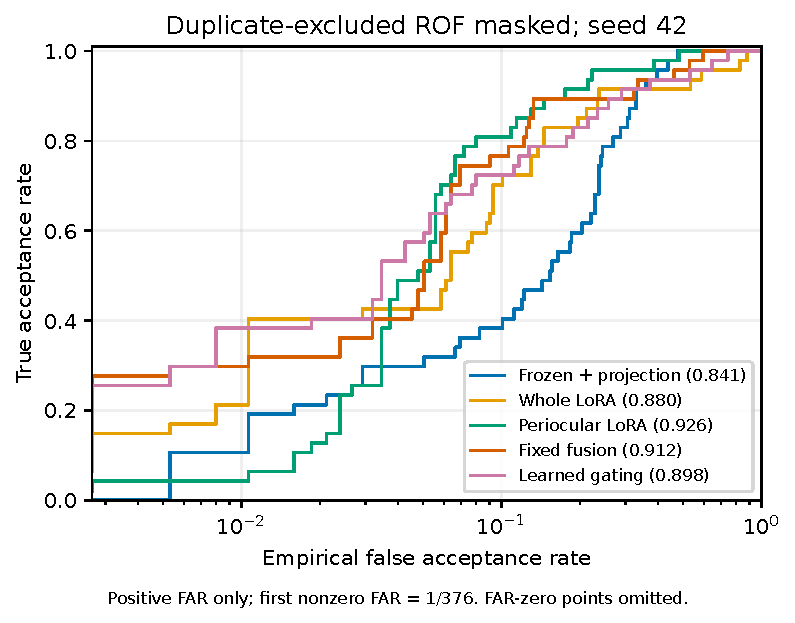
\includegraphics[width=\columnwidth]{fig_rof_masked_roc.pdf}
\caption{New masked ROF ROC (seed=42). Only positive empirical FAR values are shown. The first non-zero FAR value is 1/376. Operating points with zero FAR have been excluded from this log scale graph.}
\label{fig:checked1}
\end{figure}
As a post-hoc exploratory cohort-composition sensitivity analysis, each of the nine masked test identities was removed in turn, together with its incident comparisons, without retraining. For 8/9 subsets, periocular LoRA gave the best mean AUC.\par
Fixed fusion gives the best results in the remaining subset. The average difference between the gated and fixed fusion is negative across all subsets (-0.0243 to -0.0026). This describes sensitivity within the observed cohort; it does not establish population bias or generalisation to unseen cohorts.\par
\subsection{Sunglasses and neutral ROF verification}
With sunglasses the periocular only model performs poorly, with a mean AUC of 0.7905 compared to frozen full face (0.8780). Fixed fusion performs best (mean AUC 0.8950), closely followed by gated (0.8924) and full face LoRA (0.8913). The average difference between the gated and fixed models is -0.0026. The 95\% sensitivity interval is therefore [-0.0099, 0.0061]. Thus, there is not guaranteed improvement in performance by adding extra branches and learning a weighting combination.\par
With neutral images, learned gate fusion gives the best average AUC (0.9458) compared to fixed fusion (0.9428) and full face LoRA (0.9413). The average difference between gated and fixed fusion is 0.003. The 95\% sensitivity interval is [-0.0046, 0.0106]. Due to the small difference, there is not conclusive evidence that population performance is better in gated models. The periocular only model had a mean AUC of 0.8875. Thus, some information was lost by removing clean lower face cues. Including a neutral control in Table~\ref{tab:checked5} ensures that claims for different conditions cannot be solely made from probed images with occlusions.\par
\begin{table}[t]\centering
\caption{Results for new sunglasses ROF data. (277 Genuine and 6371 Impostors). AUC/EER/TAR values are averaged across sample seeds (standard deviation in subscript), averages taken over 3 seeds. TAR values have been derived from the ROC curves, and are not calibrated test rates.}
\label{tab:checked4}
\footnotesize\setlength{\tabcolsep}{2pt}
\sbox{\uploadedtablebox}{\begin{tabular}{lllll}\toprule
Config & AUC & EER & TAR 0.01 & TAR 0.001\\\midrule
Frozen + Projection & \shortstack{0.8780\\\ensuremath{\pm}0.003} & \shortstack{0.1774\\\ensuremath{\pm}0.004} & \shortstack{0.1095\\\ensuremath{\pm}0.002} & \shortstack{0.0132\\\ensuremath{\pm}0.004}\\
Whole LoRA & \shortstack{0.8913\\\ensuremath{\pm}0.002} & \shortstack{0.1596\\\ensuremath{\pm}0.005} & \shortstack{0.1661\\\ensuremath{\pm}0.010} & \shortstack{0.0337\\\ensuremath{\pm}0.004}\\
Periocular LoRA & \shortstack{0.7905\\\ensuremath{\pm}0.014} & \shortstack{0.2632\\\ensuremath{\pm}0.007} & \shortstack{0.0710\\\ensuremath{\pm}0.010} & \shortstack{0.0048\\\ensuremath{\pm}0.004}\\
Fixed Fusion & \shortstack{0.8950\\\ensuremath{\pm}0.002} & \shortstack{0.1531\\\ensuremath{\pm}0.008} & \shortstack{0.1564\\\ensuremath{\pm}0.012} & \shortstack{0.0144\\\ensuremath{\pm}0.006}\\
Gate Fusion & \shortstack{0.8924\\\ensuremath{\pm}0.006} & \shortstack{0.1544\\\ensuremath{\pm}0.001} & \shortstack{0.1384\\\ensuremath{\pm}0.016} & \shortstack{0.0373\\\ensuremath{\pm}0.008}\\
\bottomrule\end{tabular}}
\ifdim\wd\uploadedtablebox>\columnwidth\resizebox{\columnwidth}{!}{\usebox{\uploadedtablebox}}\else\usebox{\uploadedtablebox}\fi
\end{table}
\begin{table}[t]\centering
\caption{Results for new neutral ROF data. (570 Genuine and 15390 Impostors). AUC/EER/TAR values are averaged across sample seeds (standard deviation in subscript), averages taken over 3 seeds. TAR values have been derived from the ROC curves, and are not calibrated test rates.}
\label{tab:checked5}
\footnotesize\setlength{\tabcolsep}{2pt}
\sbox{\uploadedtablebox}{\begin{tabular}{lllll}\toprule
Config & AUC & EER & TAR 0.01 & TAR 0.001\\\midrule
Frozen + Projection & \shortstack{0.9328\\\ensuremath{\pm}0.001} & \shortstack{0.1503\\\ensuremath{\pm}0.001} & \shortstack{0.2240\\\ensuremath{\pm}0.006} & \shortstack{0.0468\\\ensuremath{\pm}0.006}\\
Whole LoRA & \shortstack{0.9413\\\ensuremath{\pm}0.002} & \shortstack{0.1237\\\ensuremath{\pm}0.003} & \shortstack{0.2269\\\ensuremath{\pm}0.063} & \shortstack{0.0193\\\ensuremath{\pm}0.005}\\
Periocular LoRA & \shortstack{0.8875\\\ensuremath{\pm}0.005} & \shortstack{0.1707\\\ensuremath{\pm}0.003} & \shortstack{0.0942\\\ensuremath{\pm}0.006} & \shortstack{0.0263\\\ensuremath{\pm}0.008}\\
Fixed Fusion & \shortstack{0.9428\\\ensuremath{\pm}0.001} & \shortstack{0.1146\\\ensuremath{\pm}0.002} & \shortstack{0.1883\\\ensuremath{\pm}0.022} & \shortstack{0.0310\\\ensuremath{\pm}0.017}\\
Gate Fusion & \shortstack{0.9458\\\ensuremath{\pm}0.003} & \shortstack{0.1122\\\ensuremath{\pm}0.007} & \shortstack{0.1965\\\ensuremath{\pm}0.024} & \shortstack{0.0205\\\ensuremath{\pm}0.005}\\
\bottomrule\end{tabular}}
\ifdim\wd\uploadedtablebox>\columnwidth\resizebox{\columnwidth}{!}{\usebox{\uploadedtablebox}}\else\usebox{\uploadedtablebox}\fi
\end{table}
\begin{figure}[t]\centering
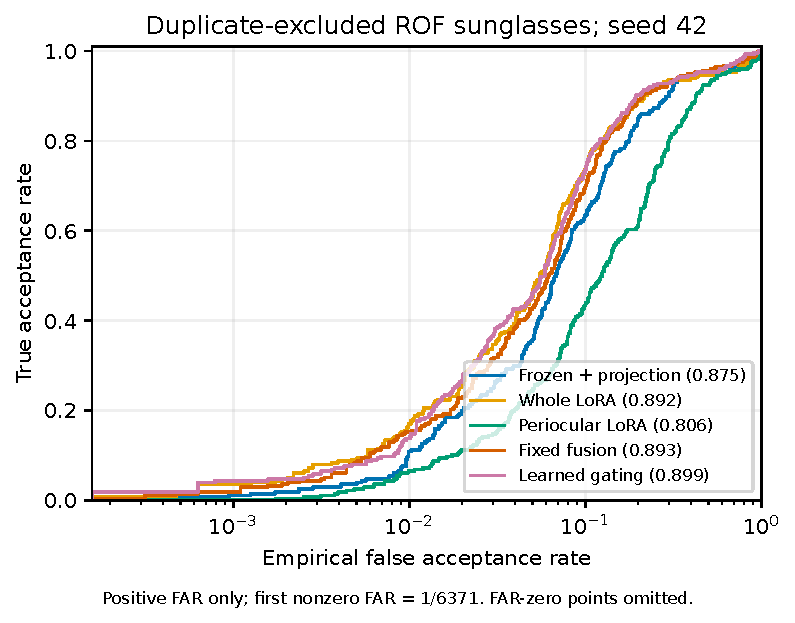
\includegraphics[width=\columnwidth]{fig_rof_sunglasses_roc.pdf}
\caption{New set of sunglasses (Seed 42). Only positive empirical FAR values are displayed. All systems use the same frozen pairs.}
\label{fig:checked2}
\end{figure}
\subsection{Known-overlap-excluded MFR2}
The best average AUC value for learned fusion is achieved at 0.9548, evaluated on 802 pairs and averaged over three seeds. The average AUC for fixed fusion was 0.9398, meaning an average improvement in AUC of 0.015 was achieved by using learned fusion over fixed fusion. The 95\% identity-resampling sensitivity interval for this improvement is [0.0044, 0.0283]. For full face LoRA models, an average AUC was achieved of 0.9360, which shows improvement over the frozen baseline model (0.8412). This improvement is larger than that in gate fusions over fixed fusions. No labels in the target domain were used in gradient updates or calibration.\par
After excluding the known exact-name overlap, the retained 802-pair results differ from the original 820-pair analysis. No known normalised exact-name overlap with ROF training remains; unknown aliases and overlap with DINOv2 pretraining cannot be ruled out. Ordered performance under known protocols can be seen from ROC results in external data. Individual thresholds from ROF validation data have been applied in order to calculate performance.\par
\begin{table}[t]\centering
\caption{Excluded known name overlap MFR2. (406 Genuine and 396 Impostors). AUC/EER/TAR values are averaged across sample seeds (standard deviation in subscript), averages taken over 3 seeds. TAR values have been derived from the ROC curves, and are not calibrated test rates.}
\label{tab:checked6}
\footnotesize\setlength{\tabcolsep}{2pt}
\sbox{\uploadedtablebox}{\begin{tabular}{lllll}\toprule
Config & AUC & EER & TAR 0.01 & TAR 0.001\\\midrule
Frozen + Projection & \shortstack{0.8412\\\ensuremath{\pm}0.006} & \shortstack{0.2496\\\ensuremath{\pm}0.008} & \shortstack{0.1453\\\ensuremath{\pm}0.013} & \shortstack{0.0041\\\ensuremath{\pm}0.003}\\
Whole LoRA & \shortstack{0.9360\\\ensuremath{\pm}0.015} & \shortstack{0.1406\\\ensuremath{\pm}0.018} & \shortstack{0.2906\\\ensuremath{\pm}0.051} & \shortstack{0.0476\\\ensuremath{\pm}0.051}\\
Periocular LoRA & \shortstack{0.9068\\\ensuremath{\pm}0.010} & \shortstack{0.1647\\\ensuremath{\pm}0.017} & \shortstack{0.2299\\\ensuremath{\pm}0.044} & \shortstack{0.1355\\\ensuremath{\pm}0.020}\\
Fixed Fusion & \shortstack{0.9398\\\ensuremath{\pm}0.005} & \shortstack{0.1445\\\ensuremath{\pm}0.016} & \shortstack{0.3415\\\ensuremath{\pm}0.067} & \shortstack{0.1741\\\ensuremath{\pm}0.016}\\
Gate Fusion & \shortstack{0.9548\\\ensuremath{\pm}0.002} & \shortstack{0.1145\\\ensuremath{\pm}0.005} & \shortstack{0.2808\\\ensuremath{\pm}0.089} & \shortstack{0.0172\\\ensuremath{\pm}0.010}\\
\bottomrule\end{tabular}}
\ifdim\wd\uploadedtablebox>\columnwidth\resizebox{\columnwidth}{!}{\usebox{\uploadedtablebox}}\else\usebox{\uploadedtablebox}\fi
\end{table}
\begin{figure}[t]\centering
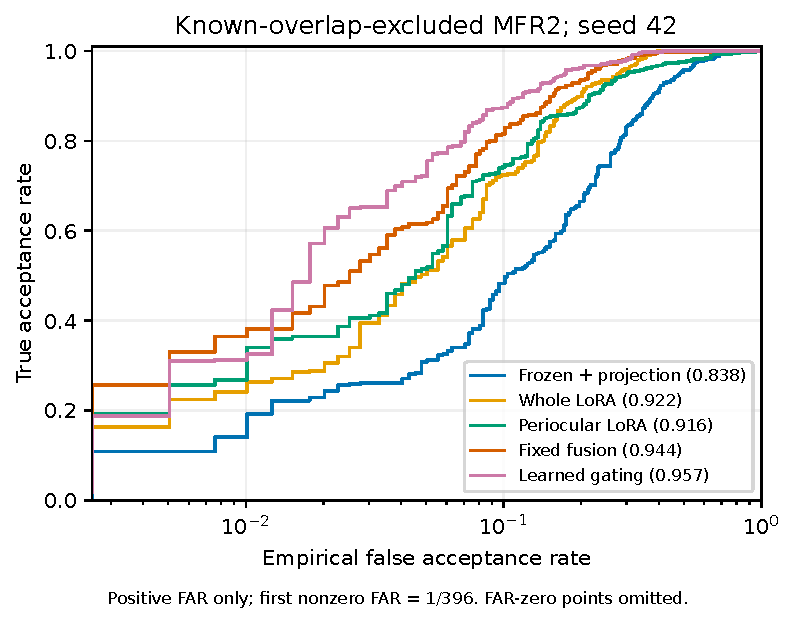
\includegraphics[width=\columnwidth]{fig_mfr2_roc.pdf}
\caption{MFR2 ROC excluding known name overlap (seed 42). Only positive empirical FAR values included. Auxiliary input is the same as in training.}
\label{fig:checked3}
\end{figure}
\subsection{Exact-conflict-excluded RMFRD}
The best exploratory results come from fixed fusion with a mean AUC of 0.7240. Next perform best learned fusion (0.7175) and then periocular LoRA (0.7132). Whole face LoRA performs with a mean AUC of 0.7045 and frozen baseline with 0.6957. The average difference is -0.0066 between gated and fixed models. The 95\% sensitivity interval is [-0.0135, 0.0004]. As 0 is within the final descriptive interval, conclusive ordering could not be determined. Thus, RMFRD labels cannot be considered independently validated.\par
A much lower AUC than MFR2 demonstrates difficulties in transfer. Although known exact conflicts have been removed, uncertainty within annotations and acquisition means strong claims cannot be made for unseen identities or deployments. Summary results for all 5 test scenarios are presented in Fig 4. Variability between seeds is presented, rather than optimum datasets.\par
\begin{table}[t]\centering
\caption{Exploratory results for excluded exact conflict RMFRD. (1038 Genuine and 20760 Impostors). AUC/EER/TAR values are averaged across sample seeds (standard deviation in subscript), averages taken over 3 seeds. TAR values have been derived from the ROC curves, and are not calibrated test rates.}
\label{tab:checked7}
\footnotesize\setlength{\tabcolsep}{2pt}
\sbox{\uploadedtablebox}{\begin{tabular}{lllll}\toprule
Config & AUC & EER & TAR 0.01 & TAR 0.001\\\midrule
Frozen + Projection & \shortstack{0.6957\\\ensuremath{\pm}0.004} & \shortstack{0.3518\\\ensuremath{\pm}0.002} & \shortstack{0.0267\\\ensuremath{\pm}0.004} & \shortstack{0.0035\\\ensuremath{\pm}0.001}\\
Whole LoRA & \shortstack{0.7045\\\ensuremath{\pm}0.010} & \shortstack{0.3507\\\ensuremath{\pm}0.011} & \shortstack{0.0324\\\ensuremath{\pm}0.009} & \shortstack{0.0045\\\ensuremath{\pm}0.001}\\
Periocular LoRA & \shortstack{0.7132\\\ensuremath{\pm}0.004} & \shortstack{0.3412\\\ensuremath{\pm}0.005} & \shortstack{0.0373\\\ensuremath{\pm}0.001} & \shortstack{0.0035\\\ensuremath{\pm}0.002}\\
Fixed Fusion & \shortstack{0.7240\\\ensuremath{\pm}0.010} & \shortstack{0.3358\\\ensuremath{\pm}0.008} & \shortstack{0.0459\\\ensuremath{\pm}0.003} & \shortstack{0.0071\\\ensuremath{\pm}0.002}\\
Gate Fusion & \shortstack{0.7175\\\ensuremath{\pm}0.012} & \shortstack{0.3356\\\ensuremath{\pm}0.010} & \shortstack{0.0421\\\ensuremath{\pm}0.004} & \shortstack{0.0083\\\ensuremath{\pm}0.002}\\
\bottomrule\end{tabular}}
\ifdim\wd\uploadedtablebox>\columnwidth\resizebox{\columnwidth}{!}{\usebox{\uploadedtablebox}}\else\usebox{\uploadedtablebox}\fi
\end{table}
\begin{figure}[t]\centering
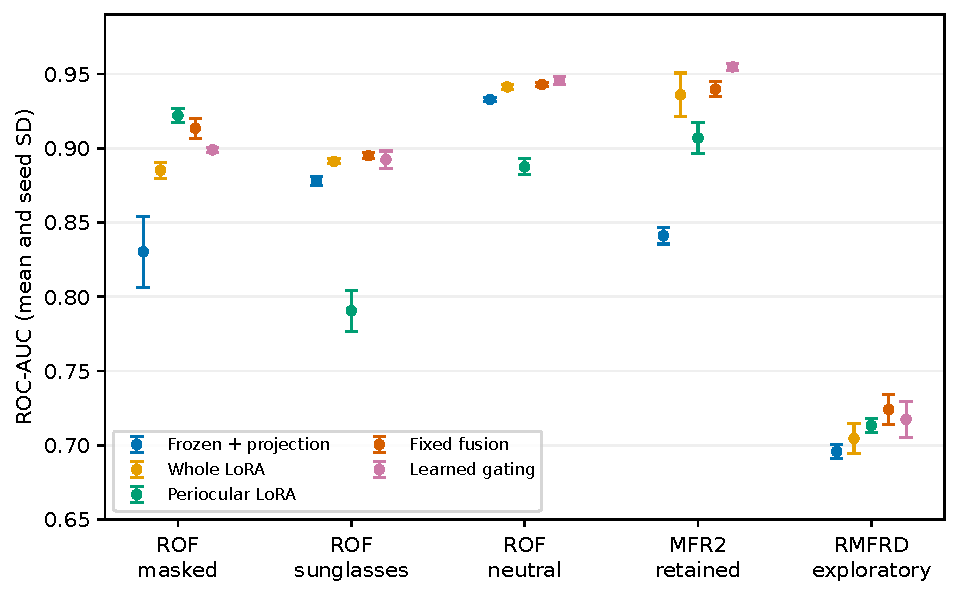
\includegraphics[width=\columnwidth]{fig_auc_cross_dataset.pdf}
\caption{Average AUC (with single sample SD from 3 seeds) for models trained on CPU. Known name overlaps are excluded in MFR2. Known exact content conflicts are excluded in RMFRD.}
\label{fig:checked4}
\end{figure}
\subsection{Validation-calibrated operating points}
Results for models with a target False Acceptance Rate (FAR) of 0.01 in validation are presented in Table~\ref{tab:checked8}. Results show mean True Acceptance Rate (TAR) and False Acceptance Rate (FAR) in testing. Count of accepts in testing for each seed given. With ROF, the same validation scenario was used. With external data sets, masked ROF validation was used. It is possible that the test FAR may be higher than the target validation FAR. In particular, testing on neutral images results in significantly higher false acceptance rates than expected from validation. If preselected thresholds are presented in a ROC curve for testing this can be misleading.\par
For a target FAR of 0.001 in validation, zero false acceptances may be observed in validation. This does not guarantee a population FAR of 0.001. For all models, complete threshold values, and counts of accepts across calibration/testing for each seed are provided in the machine readable reports. Values given for both target FARs. Calibration is done according to a set rule, and is unchanged regardless of error in testing.\par
\begin{table}[t]\centering
\caption{Gate model with target FAR of 0.01 in validation. Averages from 3 seeds. Values for TA/FA indicate number of accepts in testing for each seed in turn. Thresholds from external datasets transferred from masked ROF validation.}
\label{tab:checked8}
\footnotesize\setlength{\tabcolsep}{2pt}
\sbox{\uploadedtablebox}{\begin{tabular}{lllll}\toprule
Protocol & TAR & FAR & TA & FA\\\midrule
Masked & 0.3546 & 0.0222 & 16/18/16 & 13/5/7\\
Sunglasses & 0.1252 & 0.0089 & 37/27/40 & 74/46/50\\
Neutral & 0.5076 & 0.0325 & 278/285/305 & 491/424/585\\
MFR2 & 0.6814 & 0.0396 & 299/264/267 & 21/10/16\\
RMFRD & 0.6426 & 0.3230 & 765/569/667 & 8417/5424/6273\\
\bottomrule\end{tabular}}
\ifdim\wd\uploadedtablebox>\columnwidth\resizebox{\columnwidth}{!}{\usebox{\uploadedtablebox}}\else\usebox{\uploadedtablebox}\fi
\end{table}
\subsection{Same-branch gate controls}
To isolate the effect of fusion rule changing, the same checkpoints were used from the gate model. The features in each branch, and fusion rule, were varied by using equal weighting, average weighting (based on validation only) and permuted weighting within each branch. Results for single branch features were also obtained. Average weighting was performed based on the endpoints in validation only. Permutations were performed in each protocol using seed=42, so that unique endpoints were obtained within each protocol. No cross protocol mixing occurred. This is a post-hoc analysis, and these are not usable fusion strategies, and also not new runs of training.\par
\begin{table}[t]\centering
\caption{Average AUC values for fusion control, with same trained gate branch. Not separately trained M3 models.}
\label{tab:checked9}
\footnotesize\setlength{\tabcolsep}{2pt}
\sbox{\uploadedtablebox}{\begin{tabular}{lllll}\toprule
Protocol & Equal & Learned & Average & Permutation\\\midrule
Masked & 0.9250 & 0.8989 & 0.8946 & 0.8992\\
Sunglasses & 0.8854 & 0.8924 & 0.8934 & 0.8942\\
Neutral & 0.9421 & 0.9458 & 0.9464 & 0.9428\\
MFR2 & 0.9512 & 0.9548 & 0.9420 & 0.9391\\
RMFRD & 0.7126 & 0.7175 & 0.7181 & 0.7162\\
\bottomrule\end{tabular}}
\ifdim\wd\uploadedtablebox>\columnwidth\resizebox{\columnwidth}{!}{\usebox{\uploadedtablebox}}\else\usebox{\uploadedtablebox}\fi
\end{table}
For masked ROF images, using equal weighting gives higher average AUC (0.9250) than learned (0.8989). For sunglasses and neutral images slightly higher scores are obtained by using average weighting. For sunglasses images, permutation results in a slightly higher AUC than learned weighting (0.8942 vs 0.8924). However for MFR2 images, greater benefit is seen by using image-dependent weighting. Using learned weighting gives a mean AUC of 0.9548, whereas average and permutation give 0.9420 and 0.9391. Thus, evidence of benefit from sample dependency in weighting depends on test scenario.\par
Average weighting across seeds varies from 0.709 to 0.749 in masked ROF, and from 0.825 to 0.841 in sunglasses. Thus, more weighting occurs in the face branch for sunglasses scenarios. However, there is variability within seeds. Therefore there may be condition-dependent weighting in branches. However weighting does not indicate reliable calibrated detection, or causative detection of occlusions. Including constant auxiliary input within the bias of the first layer only has a very small effect on gate weights (max difference between recorded checkpoints of \ensuremath{1.20\times10^{-7}}). Thus, no image-specific quality information is being conveyed through auxiliary fields.\par
\begin{figure}[t]\centering
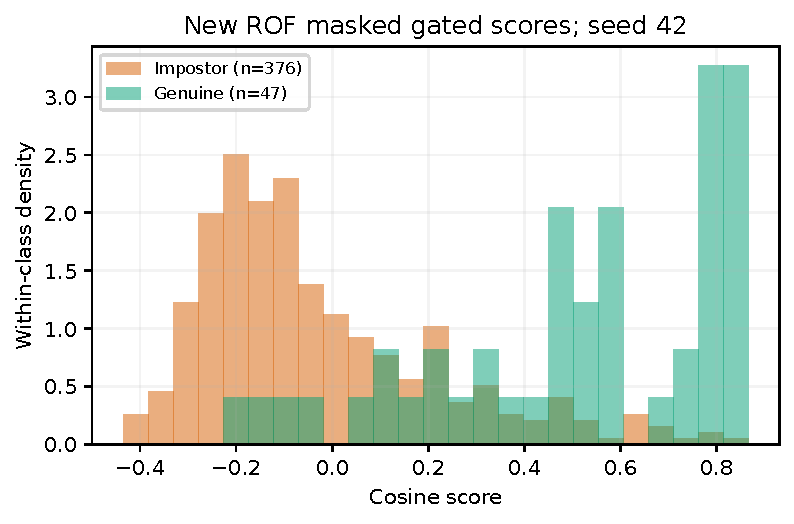
\includegraphics[width=\columnwidth]{fig_rof_masked_scores.pdf}
\caption{Gate fusion results in new masked ROF (seed 42). Shared bins. Normalisation within classes. Number of genuine and impostors visible.}
\label{fig:checked5}
\end{figure}

\subsection{Pretrained face-recognition diagnostic}
\textit{Aligned SFace diagnostic.} OpenCV SFace \cite{sface} (December 2021) was evaluated with YuNet \cite{yunet} (March 2023), five-landmark alignment, and 112-by-112-pixel native input. The detection confidence threshold was 0.8; the detection nearest the image centre was selected. No target fine-tuning was performed. Failed-pair scores were set to -1 and retained in the denominator; detected-only metrics were secondary. Table~\ref{tab:checked11} reports this aligned protocol: AUCs were 0.9399, 0.9440, 0.9991, 0.9968, and 0.8187 for masked ROF, sunglasses ROF, neutral ROF, retained MFR2, and retained RMFRD. Detection failed in 9, 48, 0, 0, and 1155 pairs, respectively. Endpoints and raw scores are recorded in the released ledger.\par
Although these results produce higher mean AUCs than new DINOv2 variants on each protocol, they are not directly comparable due to differences in pre-training data, exposure to identities, detection, alignment and objective. This shows that this ablation study does not produce state-of-the-art face verification. A controlled modern face recognition method, and independent external labels would be required to make a stronger comparative claim.\par
\begin{table}[t]\centering
\caption{Aligned SFace diagnostic with YuNet detection and five-landmark alignment. Failed pairs receive score -1 and remain in the denominator. These are not the shared-crop SFace results (Supplemental Table S3); differences in pretraining and preprocessing prevent a controlled architecture comparison.}
\label{tab:checked11}
\footnotesize\setlength{\tabcolsep}{2pt}
\sbox{\uploadedtablebox}{\begin{tabular}{lll}\toprule
Protocol & AUC & Failed Pairs\\\midrule
Masked & 0.9399 & 9\\
Sunglasses & 0.9440 & 48\\
Neutral & 0.9991 & 0\\
MFR2 & 0.9968 & 0\\
RMFRD & 0.8187 & 1155\\
\bottomrule\end{tabular}}
\ifdim\wd\uploadedtablebox>\columnwidth\resizebox{\columnwidth}{!}{\usebox{\uploadedtablebox}}\else\usebox{\uploadedtablebox}\fi
\end{table}
\textit{Shared-crop SFace preprocessing control.} The exact DINOv2 whole-face input files were resized to 112-by-112 pixels for SFace, without YuNet detection or landmark alignment. AUCs were 0.8408, 0.7775, 0.8689, 0.9513, and 0.6532 in the same protocol order (Supplemental Table S3); all 3402 unique images were extracted without failure. The two SFace protocols use different preprocessing, so their AUCs are preprocessing diagnostics rather than directly interchangeable baseline results. Neither is a matched-training comparison with DINOv2 because architecture, pretraining, resolution, and supervision differ.\par
\subsection{Paired comparisons}
All pre-defined paired comparisons from summary results are presented in Table~\ref{tab:checked12}. Negative comparisons have also been included. If difference is positive, model 1 performed better. The same number of resampled identities were applied to each model, for each of 3 seeds. Average difference calculated for each replicate. The intervals depend on the fitted checkpoints and fixed protocols, and are not confidence intervals for performance in arbitrary populations.\par
\begin{table}[t]\centering
\caption{Average differences in AUC values. 95\% sensitivity intervals from 2 endpoint identity resamplings. 1000 replicates. (G-F: Gate - Fixed fusion; W-B: Whole LoRA - Frozen base).}
\label{tab:checked12}
\footnotesize\setlength{\tabcolsep}{2pt}
\sbox{\uploadedtablebox}{\begin{tabular}{lllll}\toprule
Protocol & Comparison & Difference & Lower & Upper\\\midrule
Masked & G-F & -0.0145 & -0.0560 & 0.0144\\
Masked & W-B & 0.0549 & -0.0424 & 0.1697\\
Sunglasses & G-F & -0.0026 & -0.0099 & 0.0061\\
Sunglasses & W-B & 0.0133 & -0.0030 & 0.0366\\
Neutral & G-F & 0.0030 & -0.0046 & 0.0106\\
Neutral & W-B & 0.0085 & -0.0117 & 0.0274\\
MFR2 & G-F & 0.0150 & 0.0044 & 0.0283\\
MFR2 & W-B & 0.0948 & 0.0513 & 0.1474\\
RMFRD & G-F & -0.0066 & -0.0135 & 0.0004\\
RMFRD & W-B & 0.0088 & -0.0067 & 0.0263\\
\bottomrule\end{tabular}}
\ifdim\wd\uploadedtablebox>\columnwidth\resizebox{\columnwidth}{!}{\usebox{\uploadedtablebox}}\else\usebox{\uploadedtablebox}\fi
\end{table}
As subsets are audited, positive/negative intervals do not overcome bias in selection. Criteria for removal of data in these new runs were fixed. However, they were due to issues found in previous experiments. As retraining was prospective, direct influence of known images is removed. However this does not indicate that the local reconstructions represent an independent cohort. Due to provenance information it is easy to identify that numbers in this experiment are not from the original full case protocol.\par
\section{Discussion}
\subsection{Adaptation and regional complementarity}
In all test protocols, whole face LoRA performs better than frozen projection models, supporting hypothesis H1.\par
Depending on the area of the face shown, RQ2 is somewhat supported. Periocular LoRA has the best results in masked, but performs poorly in sunglasses and loses useful information in neutral.\par
RQ3 is less well supported. Gated models perform best in MFR2 and neutral ROF, but not in masks, sunglasses or RMFRD. Many of the comparisons included 0 within the range. Most importantly, the control experiments using the same branch show that the decision within gated models do not consistently form high quality representations. Using equal weighting in the models increased performance in masked compared to trained gated branches. Using a constant mean weighting, derived from validation only, also had competitive performance in ROF. There is no evidence to suggest that learning a gate automatically leads to increased robustness.\par
\subsection{AUC and calibration}
The AUC indicates the performance across the score range. However, in deployment a particular threshold will be selected. Improvements in AUC may lead to poor performance at strict FAR requirements. As can be seen from the calibrated counts in validation, distributional shift has occurred. The thresholds that give desired performance in validation do not necessarily give desired performance on new identities. This is especially important in the neutral tests. Many identities were repeated in enrolment and probing, meaning that large pair counts appear to be present. However, this does not necessarily mean that large amounts of independent information is present.\par
Very few genuine pairs are present in the masked test (47). As only 9 identities are present, a change in 1 genuine acceptance will change TAR by 1/47. Also, a change in 1 impostor acceptance in testing will change FAR by 1/376. Four decimal places have been added to aid manual checks, but this does not indicate that four decimal place statistical precision has been reached. Identity node resampling is a sensitivity analysis for the limited protocol. This does not indicate that more independent identities and sessions have been obtained.\par
Score distribution plots show the overlapping of genuine and impostor scores.\par
\subsection{Positioning and negative findings}
Due to differences in training data and alignment, a fair comparison of model architectures could not be made.\par
Since a constant auxiliary vector is used, care must be taken in the interpretation of results.\par
\section{Limitations and Threats to Validity}
Despite removing duplicate pairs, it cannot be guaranteed that all labels are semantically correct. Also, not all perceptual duplicates may have been identified. Despite matching annotation sources, local differences in image capture may arise. Normalised name overlaps may fail to identify all alias pairs. Public figures may have been included in pre-training in DINOv2/SFace. It is unknown how many new identities they were exposed to.\par
Only 3 initialisations were tested. Seed SD provides descriptive information. Conditional sensitivity intervals from node bootstrapping depend on the 3 trained models and frozen identity graph. Identity sampling cannot add missing capture sessions or improve mislabelled images. With 10 comparisons, no control is provided for family wise error. Due to few masked identities and limited impostors, strong claims cannot be made in terms of security in cases of very low FAR.\par
RMFRD is exploratory. Although one known overlap has been removed in MFR2, it cannot be guaranteed that all identities in MFR2 were unseen. Differences in alignment and pre-training in SFace mean that model architectures could not be fairly compared. Maximum memory usage was not recorded. Training times (wall-clock) include pauses and sleeps and therefore should not be considered as indicative of continuous processing speeds. Deterministic training was performed on CPU. Checkpoint recovery was tested within the recorded run time. Byte for byte exact replication cannot be guaranteed between versions of packages, or between different hardware.\par
\section{Reproducibility}
Mathematical checks can be made without torch, images and checkpoints.\par
\noindent\textit{Execution and reproduction details: supplemental material.}
The release contains code, manifests, hashes, derived scores, and manuscript figures; source face images and trained checkpoint binaries are excluded. No ethics committee reviewed this project, and no formal approval or exemption is claimed. The study reused existing ROF, MFR2, and RMFRD datasets downloaded from public repositories. The reviewed records do not establish individual participant consent or complete image-use permissions.\par
\section{Conclusion}
Five parameter efficient configurations, both for whole faces and periocular regions, have been compared. None of the configurations provide the best performance across all conditions. Periocular LoRA had the best performance in masked (Mean AUC = 0.9221). Fixed fusion performed best in sunglasses (0.8950) and exploratory RMFRD (0.7240). Learned fusion had the best performance in neutral ROF (0.9458) and retained MFR2 (0.9548).\par
Care should be taken when interpreting these results. Removing one identity at a time preserves the masked gated-versus-fixed direction, but results depend on cohort composition. Results are also vulnerable to pre-processing as common crops were used in SFace. Despite useful individual features being learnt by the model, optimal weighting may not have been achieved. Constant weighting models may perform well. The variation in testing FAR values could be caused by threshold calibration during validation. It has been supported that complementary information exists in different regions, but it cannot be universally claimed that security and robustness is guaranteed.\par
Archived scores, fixed protocols, and execution records support verification of the reported measurements. Stronger generalisation claims require more independent identities, matched face-specific baselines, and verified semantic labels. Data provenance and the available ethics and permissions records are described in Supplemental Section IX.\par
\section*{Funding and Competing Interests}
This research received no external funding. The author declares no competing interests.\par
\IEEEtriggeratref{27}
\begin{thebibliography}{99}
\bibitem{dinov2} M. Oquab \textit{et al.}, ``DINOv2: Learning robust visual features without supervision,'' \textit{Transactions on Machine Learning Research}, 2024.
\bibitem{lora} E. J. Hu, Y. Shen, P. Wallis, Z. Allen-Zhu, Y. Li, S. Wang, L. Wang, and W. Chen, ``LoRA: Low-rank adaptation of large language models,'' in \textit{Proc. ICLR}, 2022.
\bibitem{sphereface} W. Liu, Y. Wen, Z. Yu, M. Li, B. Raj, and L. Song, ``SphereFace: Deep hypersphere embedding for face recognition,'' in \textit{Proc. IEEE CVPR}, 2017, pp. 212--220.
\bibitem{cosface} H. Wang, Y. Wang, Z. Zhou, X. Ji, D. Gong, J. Zhou, Z. Li, and W. Liu, ``CosFace: Large margin cosine loss for deep face recognition,'' in \textit{Proc. IEEE CVPR}, 2018, pp. 5265--5274.
\bibitem{arcface} J. Deng, J. Guo, N. Xue, and S. Zafeiriou, ``ArcFace: Additive angular margin loss for deep face recognition,'' in \textit{Proc. IEEE CVPR}, 2019, pp. 4690--4699.
\bibitem{adaface} M. Kim, A. K. Jain, and X. Liu, ``AdaFace: Quality adaptive margin for face recognition,'' in \textit{Proc. IEEE CVPR}, 2022, pp. 18750--18759.
\bibitem{magface} Q. Meng, S. Zhao, Z. Huang, and F. Zhou, ``MagFace: A universal representation for face recognition and quality assessment,'' in \textit{Proc. IEEE CVPR}, 2021, pp. 14225--14234.
\bibitem{mfr2} A. Anwar and A. Raychowdhury, ``Masked face recognition for secure authentication,'' arXiv:2008.11104, 2020. [Online]. Available: \url{https://sites.google.com/view/masktheface/mfr2-dataset}
\bibitem{llecnn} S. Ge, J. Li, Q. Ye, and Z. Luo, ``Detecting masked faces in the wild with LLE-CNNs,'' in \textit{Proc. IEEE CVPR}, 2017, pp. 2682--2690.
\bibitem{rmfrd} Z. Wang, B. Huang, G. Wang, P. Yi, and K. Jiang, ``Masked face recognition dataset and application,'' \textit{IEEE Trans. Biometrics, Behavior, and Identity Science}, vol. 5, no. 2, pp. 298--304, 2023, doi: 10.1109/TBIOM.2023.3242085.
\bibitem{surveyocc} D. Zeng, R. Veldhuis, and L. Spreeuwers, ``A survey of face recognition techniques under occlusion,'' \textit{IET Biometrics}, vol. 10, no. 6, pp. 581--606, 2021.
\bibitem{from2022} H. Qiu, D. Gong, Z. Li, W. Liu, and D. Tao, ``End2End occluded face recognition by masking corrupted features,'' \textit{IEEE Trans. Pattern Anal. Mach. Intell.}, vol. 44, no. 10, pp. 6939--6952, 2022, doi:10.1109/TPAMI.2021.3098962.
\bibitem{masklearn} L. Song, D. Gong, Z. Li, C. Liu, and W. Liu, ``Occlusion robust face recognition based on mask learning with pairwise differential Siamese network,'' in \textit{Proc. IEEE/CVF ICCV}, 2019, pp. 773--782.
\bibitem{umr} F. Boutros, N. Damer, F. Kirchbuchner, and A. Kuijper, ``Self-restrained triplet loss for accurate masked face recognition,'' \textit{Pattern Recognition}, vol. 124, Art. 108473, 2022, doi: 10.1016/j.patcog.2021.108473.
\bibitem{focusface} P. C. Neto, F. Boutros, J. R. Pinto, N. Damer, A. F. Sequeira, and J. S. Cardoso, ``FocusFace: Multi-task contrastive learning for masked face recognition,'' in \textit{Proc. IEEE Int. Conf. Automatic Face and Gesture Recognition (FG)}, 2021, pp. 1--8.
\bibitem{beyondmasks} P. C. Neto, J. R. Pinto, F. Boutros, N. Damer, A. F. Sequeira, and J. S. Cardoso, ``Beyond masks: On the generalization of masked face recognition models to occluded face recognition,'' \textit{IEEE Access}, vol. 10, pp. 86222--86233, 2022, doi: 10.1109/ACCESS.2022.3199014.
\bibitem{mfr2021} F. Boutros et al., ``MFR 2021: Masked face recognition competition,'' in \textit{Proc. IEEE Int. Joint Conf. Biometrics (IJCB)}, 2021, pp. 1--10, doi: 10.1109/IJCB52358.2021.9484337.
\bibitem{insightfacemfr} J. Deng, J. Guo, X. An, Z. Zhu, and S. Zafeiriou, ``Masked face recognition challenge: The InsightFace track report,'' in \textit{Proc. IEEE/CVF ICCVW}, 2021, pp. 1437--1444.
\bibitem{hsu2022} G.-S. J. Hsu, H.-Y. Wu, C.-H. Tsai, S. Yanushkevich, and M. L. Gavrilova, ``Masked face recognition from synthesis to reality,'' \textit{IEEE Access}, vol. 10, pp. 37938--37952, 2022, doi: 10.1109/ACCESS.2022.3160828.
\bibitem{rof} M. E. Erakın, U. Demir, and H. K. Ekenel, ``On recognizing occluded faces in the wild,'' in \textit{Proc. Int. Conf. Biometrics Special Interest Group (BIOSIG)}, 2021, doi: 10.1109/BIOSIG52210.2021.9548293.
\bibitem{fbr2024} L. C. O. Tiong, D. Sigmund, C.-H. Chan, and A. B. J. Teoh, ``Flexible biometrics recognition: Bridging the multimodality gap through attention alignment and prompt tuning,'' in \textit{Proc. IEEE/CVF Conf. Computer Vision and Pattern Recognition (CVPR)}, 2024, pp. 267--276.
\bibitem{periocular} U. Park, R. R. Jillela, A. Ross, and A. K. Jain, ``Periocular biometrics in the visible spectrum,'' \textit{IEEE Trans. Inf. Forensics Security}, vol. 6, no. 1, pp. 96--106, 2011, doi: 10.1109/TIFS.2010.2096810.
\bibitem{ckd2024} Y. G. Jung, J. Park, C. Y. Low, J. C. L. Chai, L. C. O. Tiong, and A. B. J. Teoh, ``Periocular embedding learning with consistent knowledge distillation from face,'' \textit{Neurocomputing}, vol. 575, Art. 127263, 2024, doi: 10.1016/j.neucom.2024.127263.
\bibitem{ocularcrop2025} F. Alonso-Fernandez, K. Hernandez-Diaz, J. M. Buades Rubio, and J. Bigun, ``Leveraging large-scale face datasets for deep periocular recognition via ocular cropping,'' arXiv:2510.26294, 2025. [Online]. Available: \url{https://arxiv.org/abs/2510.26294}
\bibitem{perilora2026} D. Prasad, M. Deshmukh, P. Kumar, and L. K. Awasthi, ``Robust cross-spectral periocular biometric recognition using LoRA-adapted DINOv2 and quality-aware fusion,'' \textit{IETE Journal of Research}, vol. 72, no. 10, pp. 2788--2798, 2026, doi: 10.1080/03772063.2026.2695248.
\bibitem{dino} M. Caron, H. Touvron, I. Misra, H. J\'egou, J. Mairal, P. Bojanowski, and A. Joulin, ``Emerging properties in self-supervised vision transformers,'' in \textit{Proc. ICCV}, 2021, pp. 9650--9660.
\bibitem{mae} K. He, X. Chen, S. Xie, Y. Li, P. Doll\'ar, and R. Girshick, ``Masked autoencoders are scalable vision learners,'' in \textit{Proc. CVPR}, 2022, pp. 16000--16009.
\bibitem{simclr} T. Chen, S. Kornblith, M. Norouzi, and G. Hinton, ``A simple framework for contrastive learning of visual representations,'' in \textit{Proc. ICML}, 2020, pp. 1597--1607.
\bibitem{clip} A. Radford, J. W. Kim, C. Hallacy, A. Ramesh, G. Goh, S. Agarwal, G. Sastry, A. Askell, P. Mishkin, J. Clark, G. Krueger, and I. Sutskever, ``Learning transferable visual models from natural language supervision,'' in \textit{Proc. ICML}, 2021, pp. 8748--8763.
\bibitem{froundation2025} T. Chettaoui, N. Damer, and F. Boutros, ``FRoundation: Are foundation models ready for face recognition?,'' \textit{Image and Vision Computing}, vol. 156, Art. 105453, 2025, doi: 10.1016/j.imavis.2025.105453.
\bibitem{foundationcomparison2025} R. Sony, P. Farmanifard, A. Ross, and A. K. Jain, ``Foundation versus domain-specific models: Performance comparison, fusion, and explainability in face recognition,'' in \textit{Proc. IEEE/CVF ICCV Workshops}, 2025, pp. 3715--3725.
\bibitem{vpt} M. Jia, L. Tang, B.-C. Chen, C. Cardie, S. Belongie, B. Hariharan, and S.-N. Lim, ``Visual prompt tuning,'' in \textit{Proc. ECCV}, 2022, pp. 709--727.
\bibitem{prompt} B. Lester, R. Al-Rfou, and N. Constant, ``The power of scale for parameter-efficient prompt tuning,'' in \textit{Proc. EMNLP}, 2021, pp. 3045--3059.
\bibitem{adaptformer} S. Chen, C. Ge, Z. Tong, J. Wang, Y. Song, J. Wang, and P. Luo, ``AdaptFormer: Adapting vision transformers for scalable visual recognition,'' in \textit{Advances in Neural Information Processing Systems}, vol. 35, pp. 16664--16678, 2022.
\bibitem{fusionRossJain} A. Ross and A. K. Jain, ``Information fusion in biometrics,'' \textit{Pattern Recognition Letters}, vol. 24, no. 13, pp. 2115--2125, 2003.
\bibitem{quality} F. Alonso-Fernandez, J. Fierrez, and J. Ortega-Garcia, ``Quality measures in biometric systems,'' \textit{IEEE Security \& Privacy}, vol. 10, no. 6, pp. 52--62, 2012, doi: 10.1109/MSP.2011.178.
\bibitem{sface} Y. Zhong, W. Deng, J. Hu, D. Zhao, X. Li, and D. Wen, ``SFace: Sigmoid-constrained hypersphere loss for robust face recognition,'' \textit{IEEE Trans. Image Process.}, vol. 30, pp. 2587--2598, 2021, doi: 10.1109/TIP.2020.3048632.
\bibitem{yunet} W. Wu, H. Peng, and S. Yu, ``YuNet: A tiny millisecond-level face detector,'' \textit{Machine Intelligence Research}, vol. 20, no. 5, pp. 656--665, 2023, doi: 10.1007/s11633-023-1423-y.
\end{thebibliography}
\clearpage
\twocolumn[{\centering\large\bfseries Supplemental Material\par\vspace{0.5em}}]
\renewcommand{\theHsection}{supp.\arabic{section}}
\renewcommand{\theHsubsection}{supp.\arabic{section}.\arabic{subsection}}
\renewcommand{\theHtable}{supp.\arabic{table}}
\renewcommand{\theHfigure}{supp.\arabic{figure}}
\setcounter{section}{0}
\setcounter{subsection}{0}
\setcounter{table}{0}
\setcounter{figure}{0}
\renewcommand{\thetable}{S\arabic{table}}
\renewcommand{\thefigure}{S\arabic{figure}}


\noindent\textit{References: main-paper numbering.}\par
\section{Parameter efficiency}
\begin{table}[t]\centering
\caption{The total number of parameters within models and proportion trainable is given in Supplemental Table S1. Training only classifier head not included.}
\label{tab:checked2}
\footnotesize\setlength{\tabcolsep}{2pt}
\sbox{\uploadedtablebox}{\begin{tabular}{llll}\toprule
ID & Total Parameters & Trainable Parameters & (\%) Trainable\\\midrule
M0 & 87171072 & 590592 & 0.68\\
M1 & 87613440 & 1032960 & 1.18\\
M2 & 175226880 & 2065920 & 1.18\\
M3 & 175226880 & 2065920 & 1.18\\
M4 & 175424257 & 2263297 & 1.29\\
\bottomrule\end{tabular}}
\ifdim\wd\uploadedtablebox>\columnwidth\resizebox{\columnwidth}{!}{\usebox{\uploadedtablebox}}\else\usebox{\uploadedtablebox}\fi
\end{table}
M0 has 590k trainable parameters. M2 contains unused full face modality. 1,032,960 parameters are trainable. 2,065,920 is the nominal trainable parameter count of the instantiated model. The 128 class training only head has 98,432 parameters and is not included in this table. Across all adapted models, the maximum number of trainable parameters is 2.26M (1.29\%), within a double encoder model (175M). Hardware details, available runtimes, software versions, and checkpoint hashes are recorded in artifact. Maximum memory consumption was not taken.\par

\begin{table}[t]\centering
\caption{Average weighting in face branch for each protocol and seed. Standard deviation (in brackets) within endpoints. Weights are descriptives and do not indicate reliable calibrated detection.}
\label{tab:checked10}
\footnotesize\setlength{\tabcolsep}{2pt}
\sbox{\uploadedtablebox}{\begin{tabular}{llll}\toprule
Protocol & Seed 7 & Seed 42 & Seed 123\\\midrule
Masked & 0.712 (0.118) & 0.709 (0.100) & 0.749 (0.092)\\
Sunglasses & 0.841 (0.082) & 0.825 (0.083) & 0.830 (0.082)\\
Neutral & 0.773 (0.107) & 0.767 (0.096) & 0.778 (0.099)\\
MFR2 & 0.659 (0.118) & 0.632 (0.117) & 0.696 (0.103)\\
RMFRD & 0.745 (0.086) & 0.697 (0.090) & 0.775 (0.071)\\
\bottomrule\end{tabular}}
\ifdim\wd\uploadedtablebox>\columnwidth\resizebox{\columnwidth}{!}{\usebox{\uploadedtablebox}}\else\usebox{\uploadedtablebox}\fi
\end{table}
\section{Execution and recovery records}
Execution environment: PyTorch (version 2.14.0+cpu), deterministic. DINOv2 was cached. Checkpoints are atomic containing optimiser state, ordered data samples, next batch index, loss in current epoch, and random number generator states in Python, NumPy and PyTorch. Incompatible checkpoints cannot be resumed, due to manifest and source signature. In order to save a run in the serial co-ordinator, all scored hash checks must be complete. Periocular only training means that full face modality was never used in training. This means that random numbers were used differently to historical trainer. Therefore it cannot be claimed that identical bitwise optimisation was performed.\par
\section{Reproducibility details}
To reproduce this work licensed data must be obtained. The correct facial/periocular paths must be recreated. Frozen training and pair manifests must be verified. The software as recorded, and DINOv2 cache must be set up. The CPU coordinator must be run. All models will be trained for 5 epochs. Models will be scored for each protocol. Model summaries will only be created once all evaluations have been performed. File locking has been implemented to prevent multiple instances of the coordinator running. Multiple runs will produce verified complete runs. If the experiment is interrupted, it will resume from a checkpoint of the atomic optimiser and random number generator. Face images, pre-trained weight binaries and approximately 8.6 GB of newly trained checkpoints are not included. Checksums of these files are provided for local lineage checking. To reproduce inference, access to binaries must be provided.\par
Mathematical checks can be made without torch, images and checkpoints. The verification script in this repository recreates ROC scores, checks alignment and checksums of pairs, recalculates mean/SD of seeds, and checks values in the table of the manuscript. 90 historic metric files, sensitivities and corrected historic MFR2 inferences have been saved. If all of these pass, all files are internally consistent. However, no guarantees can be made that this work is novel, accepted for publication, and that images have semantically correct labels.\par
Historic versions of this manuscript and follow-up work can be found in the history folder. Claims or numerically tabulated data within these files are now out-of-date with the full CPU experiment in this paper. No new training is represented by filtered scores in historic files. Incomplete training or smoke runs do not produce headline tables. Large blocks of text and vector figures in both IEEE and arXiv are re-created together using complete evidence from results.\par
\section{Additional interpretation and result records}
In all test protocols, whole face LoRA performs better than frozen projection models, supporting hypothesis H1. The greatest improvements were seen in MFR2 and masked ROF. However, smaller improvements were found in RMFRD. Supervised adaptation thus appears to be beneficial in this experiment. It cannot be determined that adapting general visual encoders (as opposed to face specific pre-trained models) is beneficial in this experiment.\par
Depending on the area of the face shown, RQ2 is somewhat supported. Periocular LoRA has the best results in masked, but performs poorly in sunglasses and loses useful information in neutral. Therefore H2 is only somewhat supported. Upper face features provide useful information for distinguishing between subjects in lower face occlusion scenarios. However, they do not provide a good representation in all 3 conditions. Using fixed fusion provides a good baseline since information in both regions can be preserved without learning a weighting policy.\par
From results in SFace, it appears that greater ranking performance can be achieved by training the model specifically on faces. However, due to differences in training data and alignment, a fair comparison of model architectures could not be made. Therefore this work should be considered as an ablation study and study of reproducibility. In order to claim competition within face recognition, comparisons must be made with equivalent baseline models, with more identities and verified labels.\par
Since a constant auxiliary vector is used, care must be taken in the interpretation of results. As input descriptors are provided, no measure of variable quality is present in this experiment. Although the gate can react to embeddings, no evidence can be provided that quality cues improve performance. Future work using quality cues should be designed with validated descriptors and controlled ablation studies on descriptors. Evaluation criteria should also be fixed before investigation.\par
Records for 15 models in the grid have been included. 120 ordered raw-score files across 8 validation/test/external protocols. Evaluation reports, final training progression information, checksums of checkpoints and a table summarising 5 conditions with 25 rows. 10 comparisons of AUC in pairs with 3 seeds. Variance in AUC between seeds, bootstrap and conditional confidence intervals is included. Fixed versions of trainer, evaluator, common utilities, models and metrics have been included. Checksums are provided for each. If any of these sources change, execution signatures will become invalid.\par
\section{Same-branch comparison context}
As different weights are applied in the fixed and gated fusion models, different features are being learnt in each branch. By applying different weights to the gated models, but keeping the same branches, it was found that equal weighting in the gated branches performs better than learned weighting in masked ROF pairs. This analysis allows understanding of whether representations are useful, or inferences are useful. However, no assumptions are made on whether representations and inferences will be useful in tandem.\par
\section{Extended interpretation and source-image review}
The methods used to produce fusion, LoRA and weighted models are well known. Given the methods proposed in FRoundation and recent implementations using DINOv2-LoRA periocular [25, 30], it can no longer be claimed that the novel contribution of this work is adaptation within the backbone model. However, it is still valuable to understand whether the same level of robustness can be achieved using regional features, weights and thresholds. If two joint models perform competitively, it cannot be concluded that the weight adaptation is responsible for the performance difference. Having same branch control models provides a better indication of this.\par
Score distribution plots show the overlapping of genuine and impostor scores. However, no information on which identities or why errors were made can be seen. Manual inspection of labelled identities in licensed source data must be performed to make qualitative decisions. From retaining manifests and exclusion ledgers, this can be done without distributing private or restricted face images in the repository.\par
Since a constant auxiliary vector is used, care must be taken in the interpretation of results. As input descriptors are provided, no measure of variable quality is present in this experiment. Although the gate can react to embeddings, no evidence can be provided that quality cues improve performance.\par

\section{Inference architecture}
\begin{figure}[t]\centering
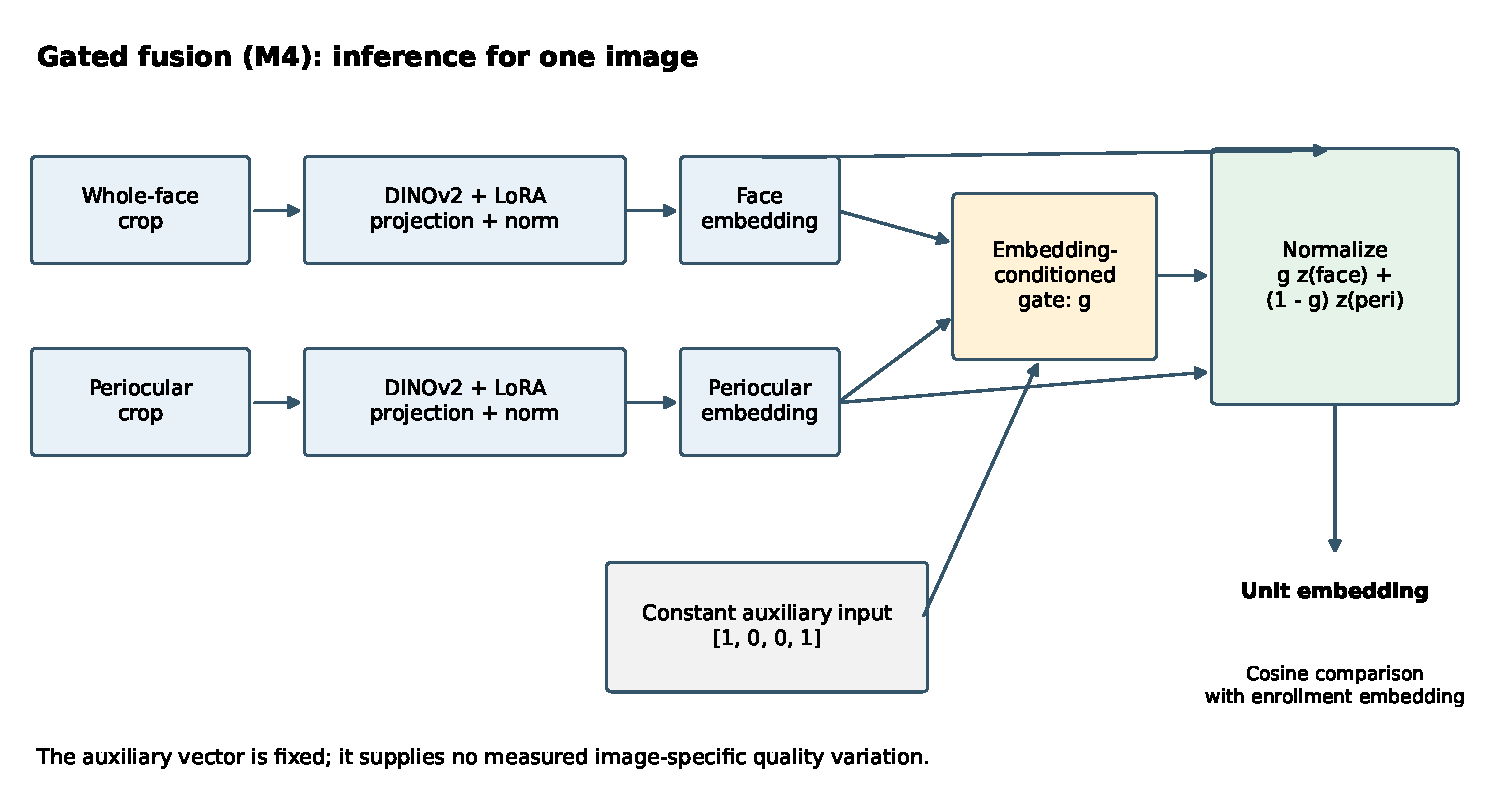
\includegraphics[width=\columnwidth]{fig_gated_architecture.pdf}
\caption{Gated-fusion inference path for one image. Both branch embeddings and the constant auxiliary vector feed the gate; the weighted mixture is normalised. The enrolment image follows the same model before cosine comparison. The training-only identity classifier is omitted from the inference path.}\label{fig:supparchitecture}\end{figure}


\section{SFace preprocessing controls}
Shared-crop SFace preprocessing control. The exact DINOv2 whole-face input files were resized to 112-by-112 pixels for SFace, without YuNet detection or landmark alignment. AUCs were 0.8408, 0.7775, 0.8689, 0.9513, and 0.6532 in the same protocol order (Supplemental Table S3); all 3402 unique images were extracted without failure. The two SFace protocols use different preprocessing, so their AUCs are preprocessing diagnostics rather than directly interchangeable baseline results. Neither is a matched-training comparison with DINOv2 because architecture, pretraining, resolution, and supervision differ.\par
\begin{table}[!ht]\centering\footnotesize\setlength{\tabcolsep}{2pt}
\caption{Separate SFace preprocessing protocols on the same retained pair lists. AUCs include failed pairs at score -1. Failed-pair counts are shown separately for each protocol. Table IX of the main paper reports only the aligned diagnostic.}
\label{tab:sfaceshared}\begin{tabular}{lrrrr}\toprule
Protocol & Aligned AUC & Failed & Shared AUC & Failed\\\midrule
Masked ROF & 0.9399 & 9 & 0.8408 & 0\\
Sunglasses ROF & 0.9440 & 48 & 0.7775 & 0\\
Neutral ROF & 0.9991 & 0 & 0.8689 & 0\\
MFR2 & 0.9968 & 0 & 0.9513 & 0\\
RMFRD & 0.8187 & 1155 & 0.6532 & 0\\
\bottomrule\end{tabular}\end{table}

\section{Data provenance and ethics records}
This study uses existing ROF, MFR2, and RMFRD datasets. Project workflows and captured run paths identify Kaggle-hosted execution copies; the original sources are the ROF repository, the MFR2 maintainer page, and the RMFRD repository. The local ROF annotation snapshot matches the audited upstream files, but a complete image-acquisition log was unavailable. Source identifiers and exclusion ledgers are retained.\par
The ROF repository carries an MIT license for software and associated documentation. The MFR2 maintainer page mentions a Creative Commons license without identifying its specific version or terms in the inspected text. The inspected RMFRD README describes web collection and supplies downloads, but an explicit image-use license was not located there. These records do not establish permission for every underlying photograph or a definitive redistribution rule for every image. The release therefore excludes source face-image binaries and trained checkpoint binaries; it provides code, manifests, hashes, derived scores, and manuscript figures.\par
No project-specific institutional approval, formal exemption, or participant-consent documentation was located in the records reviewed. This is a documentation limit; it does not establish that review was unnecessary or that consent was absent. No approval number, exemption, consent claim, or blanket image permission is inferred from public availability. The factual ethics-review determination and outstanding dataset/image-use permissions remain unresolved.\par
Source records checked on 22 November 2026: \href{https://github.com/ekremerakin/RealWorldOccludedFaces}{ROF repository}, \href{https://github.com/ekremerakin/RealWorldOccludedFaces/blob/main/LICENSE}{ROF license}, \href{https://sites.google.com/view/masktheface/mfr2-dataset}{MFR2 maintainer page}, \href{https://github.com/X-zhangyang/Real-World-Masked-Face-Dataset}{RMFRD repository}.\par

\end{document}
